\documentclass[ratio=169]{beamercours}

\captionsetup[table]{font=small}
\DeclareMathOperator{\tree}{Tree}
\DeclareMathOperator{\leaves}{Leaves}
\DeclareMathOperator{\stack}{Stack}
\DeclareMathOperator{\push}{Push}
\DeclareMathOperator{\apply}{Apply}
\def\rrrevo{\texttt{random\_evolve}}
\DeclareMathOperator{\revo}{Evolve}
\DeclareMathOperator{\coll}{Collision}
\def\mathbox#1#2{\parbox{#1}{\centering $#2$}}

\algnotext{EndWhile}
\algnotext{EndIf}
\algnotext{EndFor}

\def\mT{\mathcal{T}}
\def\P{\mathbb{P}}

\definecolor{vulm}{HTML}{7d1dd3}
\definecolor{yulm}{HTML}{ffe500}

\title{Generating Diachrony}
\author{Matthieu \textsc{Boyer}}

\tikzcdset{arrows={no head}, labels={description}}

\begin{document}
\begin{frame}
\begin{tikzpicture}[overlay,remember picture]
  \end{tikzpicture}
  \begin{tikzpicture}[remember picture, overlay]
          \node[yshift=-\headheight - 4pt] (upperleft) at (current page.north west) {};
                 \path[fill opacity=.5, fill tile picture={%
                     \node[inner sep=0pt,outer sep=0pt] {\usebox{\tileone}};
     }] (upperleft) rectangle (current page.south east);
        \node [inner sep=0pt, anchor=north, yshift=.1\paperheight] at (current page.north) {};
		\node [anchor=north, rectangle, fill=vulm!50, fill opacity=1, text opacity=1, text width=.9\paperwidth, minimum width=\paperwidth, yshift=-\headheight - 8pt, minimum height=.35\paperheight, inner sep=3pt] (title) at (current page.north) {\centering %
			{\Large\sc Language\, Evolution\, and\, Diachrony\, Generation\par}
                \vspace{5pt}
                {Research Project Report\par}
                \vspace{5pt}
			{Matthieu \textsc{Boyer}\par}};
        \node [anchor=north east, rectangle, fill=yulm!10, fill opacity=.5, text opacity=1, yshift=-.017\paperheight, xshift=-.1\paperwidth] at (title.south) {
\includegraphics[width=.3\linewidth]{logo_lattice}};
        \node [anchor=north west, rectangle, fill=yulm!10, fill opacity=.5, text opacity=1, xshift=+.1\paperwidth, yshift= -.017\paperheight] at (title.south) {\includegraphics[width=.3\linewidth]{~/Documents/ETUDES/ENS/ens_psl}};
        \node [anchor=south, yshift=\footheight + 4pt, minimum width=\paperwidth, text width=0.9\paperwidth, rectangle, fill=yulm!10, fill opacity=.5, text opacity=1] at (current page.south) {\centering %
                \vspace{3pt}
                {\sc Laboratoire\, Lattice \par}
                \vspace{4pt} %
                {\sc CNRS --- ENS-PSL --- Université Sorbonne Nouvelle\par}
                \vspace{6pt} %
                {Under supervision of Mathieu \textsc{Dehouck}\par}};
  \end{tikzpicture}

\end{frame}

\begin{frame}
	\frametitle{Introduction}
	Few database available in diachrony:
	\begin{itemize}
		\item The Index Diachronica \cite{index}
		\item The $\mathcal{E}$vosem \cite{evosem}
	\end{itemize}
	There is a need for less localized data.
\end{frame}

\section{Idea}
\subsection{One Language Evolution}
\begin{frame}[allowframebreaks, fragile]
	\frametitle{Evolution as Random Trees}
Consider a language $L_{0}$, which we will call our \emph{base language}.
\begin{category}[]
	&[-24pt] L_{0}\ar[d] &[-24pt] &[2cm] &[-12pt] L_{0}\ar[d]\ar[dl]\ar[dr] &[-12pt] &[-24pt]\\
	& L_{1, 0}\ar[dl]\ar[dr] & & L_{1, 0}\ar[d] & L_{1, 1}\ar[d] & L_{1, 2}\ar[d]\ar[dr] &\\
	L_{2, 0} & & L_{2, 1} & L_{2, 0} & L_{2, 1} & L_{2, 2} & L_{2, 3}
\end{category}

\framebreak

\begin{algorithm}[H]
	\caption{One Language Evolution}
	\label{al1evo}
	\begin{algorithmic}
		\State {$leaves \gets \{L_{0}\}$}
		\State {$\mT \gets \tree\left(L_{0}, \emptyset\right)$}
		\For {$n \leq \texttt{Epochs}$}
		\For {$l \in \leaves\mT$}
		\State {$S \gets \revo l$}
		\State {$l \gets \tree\left( l, S \right)$} \Comment{Here $\mT$ is modified in place.}
		\EndFor
		\EndFor
		\Return $\mT$
	\end{algorithmic}
\end{algorithm}
\end{frame}

\begin{frame}[allowframebreaks, fragile]
	\frametitle{Specification of $\revo$}
	We want to choose between \emph{evolution types} ($\phi, \sigma, \tau, \lambda$) at computation:
\begin{category}[]
	&[-24pt] L_{0}\ar[d, "\tau"] &[-24pt] &[2cm] &[-12pt] L_{0}\ar[d, "\tau"]\ar[dl, "\phi"]\ar[dr, "\phi"] &[-12pt] &[-24pt]\\
	& L_{1, 0}\ar[dl, "\sigma"]\ar[dr, "\phi"] & & L_{1, 0}\ar[d, "\tau"] & L_{1, 1}\ar[d, "\phi"] & L_{1, 2}\ar[d, "\lambda"]\ar[dr, "\sigma"] &\\
	L_{2, 0} & & L_{2, 1} & L_{2, 0} & L_{2, 1} & L_{2, 2} & L_{2, 3}
\end{category}

\framebreak

We want $\revo$ to be \emph{easily revertible}:
\begin{equation*}
	\P\left( \revo\left(l_{1}\right) = l_{2} \right) \neq 0 \Leftrightarrow \P\left( \revo\left( l_{2} \right) = l_{1} \right) \neq 0
\end{equation*}
\end{frame}

\subsection{Two Language Evolution}

\begin{frame}[allowframebreaks, fragile]
	\frametitle{Collision Hypothesis}
We assume language interacting create evolutions:
\begin{category}
	L_{0, 1}\ar[dr, "\phi"]\ar[d, "\tau"] &[-24pt] &[-24pt] L_{0, 2}\ar[dl, "\sigma"]\ar[d, "\lambda"]\\
	L_{1, 1} & L_{1, 2} & L_{1, 3}
\end{category}

\framebreak

\begin{algorithm}[H]
	\caption{Two Language Evolution}
	\label{alg2evo}
	\begin{algorithmic}
		\State {$\mT \gets \tree\left(L_{0}, \emptyset\right)$}
		\For {$n \leq \texttt{Epochs}$}
		\For {$l \in \leaves\mT$}
		\State {$S \gets \revo l$}
		\State {$\push\left(\stack, l \gets l \cup \tree\left( l, S \right)\right)$}
		\EndFor
		\For {$l \in \leaves\mT$}
		\State {$l^{\dag} \gets \mP_{l}\left( \leaves\mT \right)$}
		\State {$S \gets \coll\left( l, l^{\dag} \right)$}
		\State {$\push\left( \stack, l\gets l \cup \tree\left( l, S \right) \right)$}
		\EndFor
		\State {$\apply(\stack)$}
		\EndFor
		\Return $\mT$
	\end{algorithmic}
\end{algorithm}
\end{frame}

\begin{frame}
	\frametitle{Specification of $\coll$}
	$\coll$ should:
	\begin{itemize}[<+->]
		\item be \emph{easily revertible}.
		\item provide a way to choose collision type, for each parent.
		\item take \emph{linguistic} proximity of the parents into account.
		\item take the probability distribution $\mP$ as the strength of the collisions.
	\end{itemize}
\end{frame}


\begin{frame}[allowframebreaks]
	\frametitle{A Manifold of Languages}
	$\mP_{l}$ models the probability of interaction with $l$.
	Defining a \emph{geographical} embedding gives:
	\begin{equation*}
		\mP_{l} \propto \frac{1}{d_{l}\left( x \right)}
	\end{equation*}

	\framebreak

	\begin{itemize}
		\item The simplex, that is, $d_{l}(x) = 1$ for all $l, x$.
		\item $\R^{3}$, with the $\ell^{2}$ distance.
		\item The $2$-sphere $\S^{1}$ where each language is a pair$\lambda, \phi$:
	      \begin{equation*}
		      d_{\left( \theta_{1}, \lambda_{1} \right)}\left( \theta_{2}, \lambda_{2} \right) = \arccos\left( \sin \left(\phi_{1}\right) \sin\left( \phi_{2} \right) + \cos\left( \phi_{1} \right)\cos\left( \phi_{2} \right)\cos\left( \lambda_{2} - \lambda_{1} \right) \right)
	      \end{equation*}
	\end{itemize}

	\framebreak

	We suppose a language only interacts with languages from the same epoch, for now.
	We could add a new dimension to the manifold to modelize time.

	Moreover, we are not required to use a metric but simply a positive separated function.

\end{frame}

\section{Results}
\begin{frame}[allowframebreaks, fragile]
	\frametitle{Implemented}
	We worked using a modular structure:
	\begin{itemize}
		\item A tree generation module
		\item A \emph{linguistical} observable
		\item A \emph{geographical} observable
	\end{itemize}
	We have implemented all 3 previously defined \emph{geographical} observable.

	\framebreak

	We only have a lexicon observable:
	\begin{category}
		\mathbox{.2\textwidth}{\mL_{0, 0} = \left( L_{0}, \mathcal{G}_{0, 0} \right)}\ar["\lambda", d]\ar["\lambda", dr]\ar["\lambda", drr, dashed, bend left] &[-12pt] &[-12pt] &[-12pt] \mathbox{.2\textwidth}{\mL_{0, 1} = \left( L_{1}, \mathcal{G}_{0, 1} \right)}\ar["\lambda", d]\ar["\lambda", dl]\ar["\lambda", dll, dashed, bend right]\\
	\mathbox{.2\textwidth}{\mL_{1, 0} = L_{0} \setminus \{w\} \cup \{w'\}, \revo\mathcal{G}_{0, 0} }
	& \mathbox{.2\textwidth}{\mL_{1, 1} = L_{0} \setminus \left\{ w_{\leq k}\right\} \cup \left\{ u_{\leq k'} \right\}, \mathcal{G}_{0, 0} \to \mathcal{G}_{0, 1}}
	& \mathbox{.2\textwidth}{\mL_{1, 1}' = L_{1} \setminus \left\{ u_{\leq l}\right\} \cup \left\{ w_{\leq l'} \right\}, \mathcal{G}_{0, 1} \to \mathcal{G}_{0, 0} }
	& \mathbox{.2\textwidth}{\mL_{1, 2} =  L_{1} \setminus \{u\} \cup \{u'\}, \revo\mathcal{G}_{0, 1} }
\end{category}

	\framebreak

	For our probabilities, we set thresholds:
	\begin{itemize}
		\item $1 - \alpha$ representing our random evolution probability;
		\item $1 - \beta$ representing our collision generation probability.
	\end{itemize}

	Our problem is then to find \emph{optimal} parameters $\alpha, \beta, \revo, \coll$ and distribution $\mP$.
\end{frame}

\begin{frame}[allowframebreaks]
	\frametitle{Performance Checking}
	We use the $\mathcal{E}$vosem project \cite{evosem} as a lexical bank:
	\begin{itemize}
		\item Our base languages are two proto-families, Germanic and Indo-European which
derived in modern French, German, English, Dutch, Spanish, Italian and Danish.
		\item Accuracy is computed by the $\ell^{2}$ distance between subsets of the dialexification matrices.
		\item Limitation of randomness is done by repetition of the experiments, though there are $\O\left( 3^{7d} \right)$ submatrices.
	\end{itemize}

	\framebreak

	However, our algorithm is quite slow. Assuming:
	\begin{itemize}
		\item $\revo$ is done in constant time (false for phonetics, for example).
		\item $\coll$ is done in constant time.
		\item Computing $d\left( x, y \right)$ is done in constant time.
		\item Loss computation is in constant time.
	\end{itemize}
	we get a complexity in $\O\left( 3^{2d}k \right)$ for $d$ epochs and $k$ base languages, to multiply by the number of repetitions and parameters.
\end{frame}

\begin{frame}[allowframebreaks]
	\frametitle{Results}
	We take for base languages for the euclidean space:
	\begin{equation*}
		\left( \begin{pmatrix}
	1\\
	0\\
	0
\end{pmatrix}, \begin{pmatrix}
	0\\
	1\\
	0
\end{pmatrix}\right)
	\end{equation*}
	and for the sphere $\S^{1}$ we take the GPS coordinates of Paris and Berlin.

	\framebreak

\begin{figure}[H]
	\centering
	\hfill
	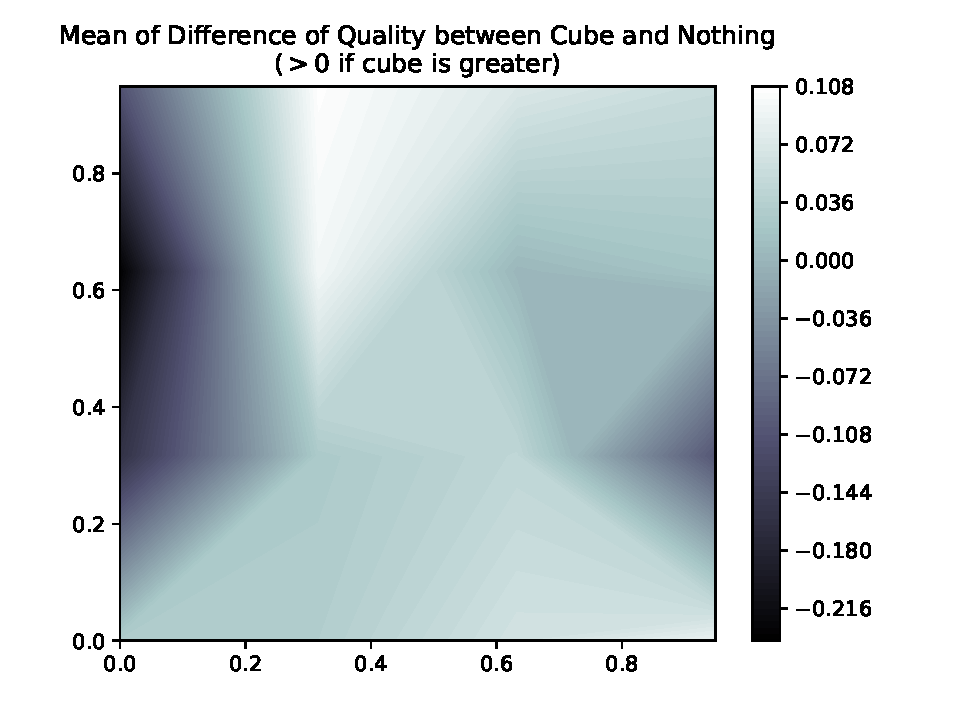
\includegraphics[width=\textwidth]{../Figures/qual_diff_cube_none}
	\caption{Plot of computed differences in accuracy between the euclidean space geography and no geography. Variance is around $\sqrt{2.10^{-2}}$.}
	\label{cubenone}
\end{figure}

	\framebreak


	\begin{figure}[h]
	\centering
	\hfill
	\begin{minipage}{.45\textwidth}
		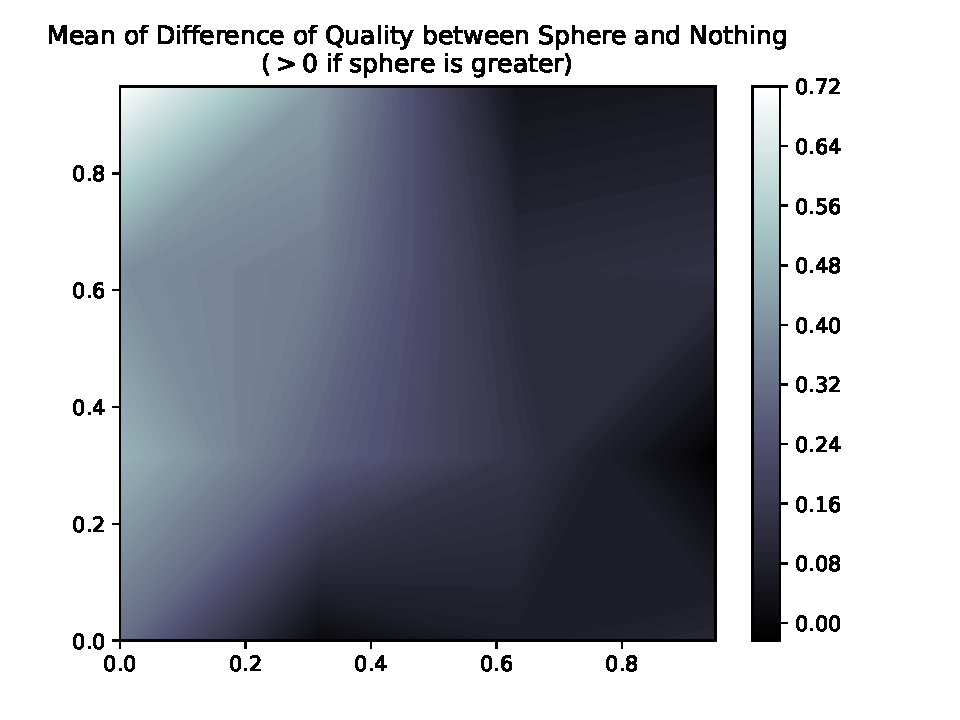
\includegraphics[width=\linewidth]{../Figures/qual_diff_sphere_none}
		\caption{Plot of computed differences in accuracy between the $\S^{1}$ sphere and no geography.}
	\label{nonesphere}
	\end{minipage}
	\hfill
	\begin{minipage}{.45\textwidth}
		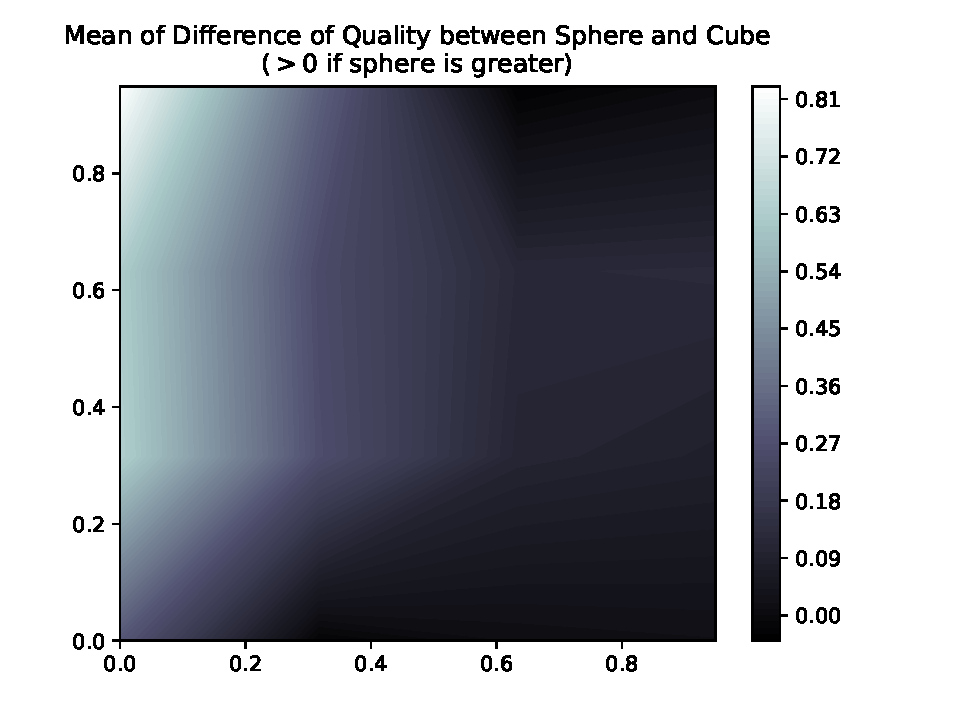
\includegraphics[width=\linewidth]{../Figures/qual_diff_sphere_cube}
	\caption{Plot of computed differences in accuracy between the euclidean space geography and the $\S^{1}$ sphere.}
	\label{cubesphere}
	\end{minipage}
	\hfill
	\end{figure}

\end{frame}

\begin{frame}[t]
	\frametitle{References}
	\bibliography{report}
	\bibliographystyle{alpha}
\end{frame}

\end{document}
